\section{Introduction}
    In this implementation, in order to demonstrate how the monitoring system works instead of using actual sensors, a data generator has been used and it simulates reading of sensors (such as humidity, temperature and electricity).

\section{Methodology}
A data generator should have a random yet realistic pattern for effective system testing, so just using a simple random number would be insufficient. Therefore, in this thesis a controlled version of choosing a random number was used to mimic some parts of real-world criteria and avoid sudden changes. The methodology for this process can be seen in the accompanying flowchart \ref{chart:data_gen}.

    \begin{figure}
        \centering
        \captionsetup{type=figure}
        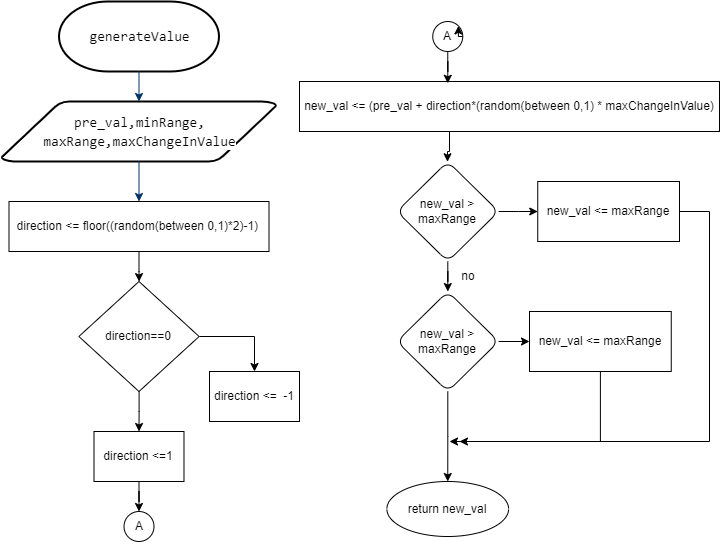
\includegraphics[width=1\textwidth]{flowchart_data_gen}
        \caption{Flowchart of data generator}
        \label{chart:data_gen}
    \end{figure}
\section{Results}
    As discussed in the methodology section, the program was implemented, and the generated values tested with different parameters was saved and reported as line charts in the subsequent sections.
    \subsection{Generated temperature sensor data}
        \begin{itemize}
            \item Parameters
                \begin{description}
                    \item[Starting Temperature sensor Value:] 22
                    \item[Minimum Possible Temperature sensor value:] 18
                    \item[Maximum Possible Temperature sensor value:] 27
                    \item[Maximum Possible Change in an iteration:] 0.5
                \end{description}
            \item Results can be seen in figure \ref{fig:gen_temperature}
                \begin{figure}
                    \centering
                    \captionsetup{type=figure}
                    \begin{subfigure}[b]{0.45\textwidth}
                        \centering
                        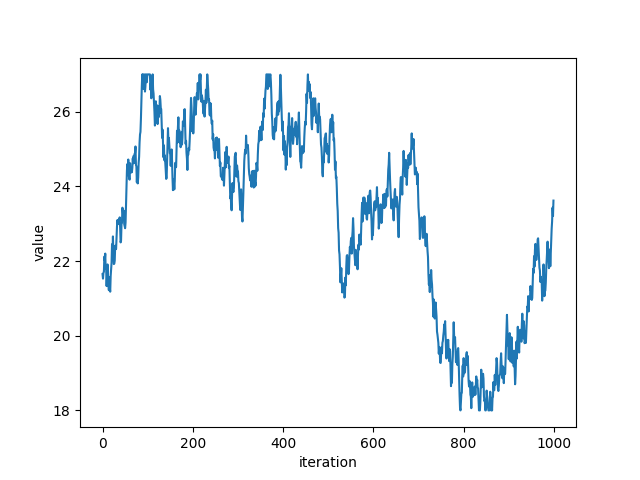
\includegraphics[width=\textwidth]{linechart_data_gen_temperature1000i}
                        \caption{For 1000 iterations}
                        \label{chart:gen_temperature_1000}
                    \end{subfigure}
                    \hfill
                    \begin{subfigure}[b]{0.45\textwidth}
                        \centering
                        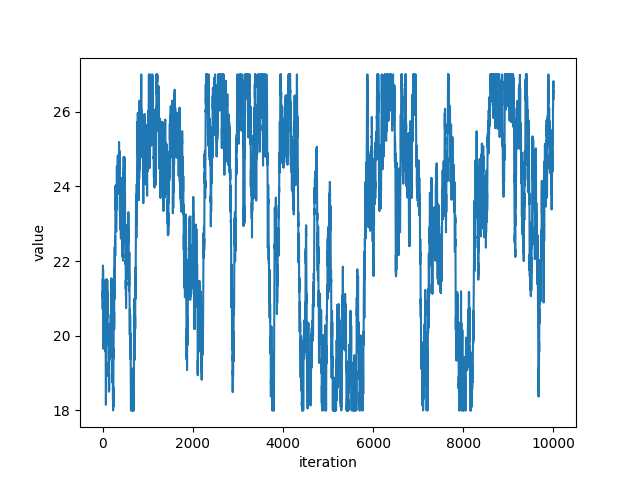
\includegraphics[width=\textwidth]{linechart_data_gen_temperature10000i}
                        \caption{For 10000 iterations}
                        \label{chart:gen_temperature_10000}
                    \end{subfigure}
                    
                    \caption{Sample generated temperature sensor data }
                    \label{fig:gen_temperature}
                \end{figure}
            \end{itemize}
            \subsection{Generated humidity sensor data}
                \begin{itemize}
                    \item Parameters
                        \begin{description}
                            \item[Starting humidity sensor value:] 55
                            \item[Minimum possible humidity sensor value:] 40
                            \item[Maximum possible humidity:] 60
                            \item[Maximum possible Change in an iteration:] 0.5
                        \end{description}
                    \item Results can be seen in figure \ref{fig:gen_humidity}
                        \begin{figure}
                            \centering
                            \captionsetup{type=figure}
                            \begin{subfigure}[b]{0.45\textwidth}
                                \centering
                                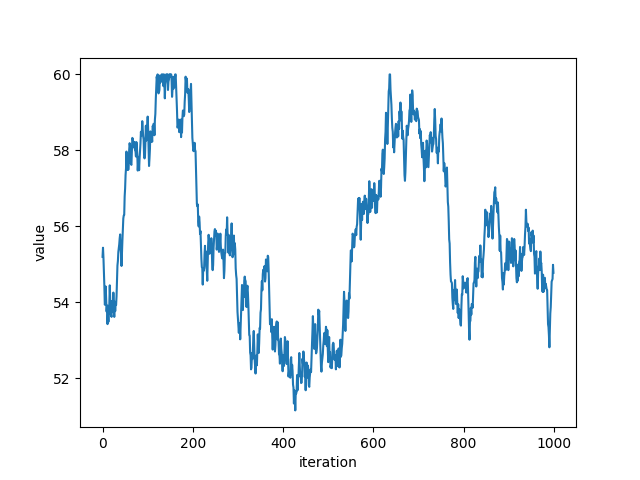
\includegraphics[width=\textwidth]{linechart_data_gen_humidity1000i}
                                \caption{For 1000 iterations}
                                \label{chart:gen_humidity_1000}
                            \end{subfigure}
                            \hfill
                            \begin{subfigure}[b]{0.45\textwidth}
                                \centering
                                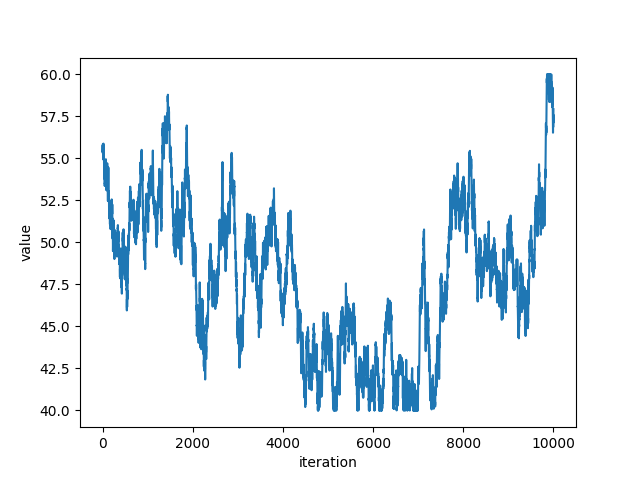
\includegraphics[width=\textwidth]{linechart_data_gen_humidity10000i}
                                \caption{For 10000 iterations}
                                \label{chart:gen_humidity_10000}
                            \end{subfigure}
                            
                            \caption{Sample generated humidity sensor data }
                            \label{fig:gen_humidity}
                        \end{figure}
                    \end{itemize}
                \subsection{Generated dust sensor data}
                    \begin{itemize}
                        \item Parameters
                            \begin{description}
                                \item[Starting dust sensor Value:] 220
                                \item[Minimum possible dust sensor value:] 208
                                \item[Maximum possible electricity dust sensor value:] 264
                                \item[Maximum possible change in an iteration:] 1
                            \end{description}
                        \item Results can be seen in figure \ref{fig:gen_dust}
                            \begin{figure}
                                \centering
                                \captionsetup{type=figure}
                                \begin{subfigure}[b]{0.45\textwidth}
                                    \centering
                                    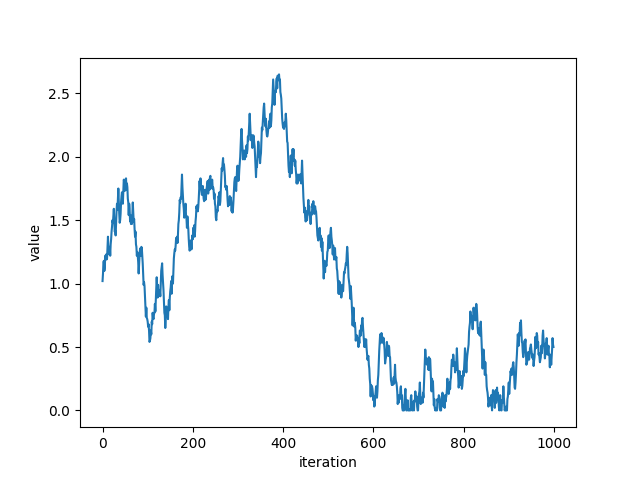
\includegraphics[width=\textwidth]{linechart_data_gen_dust1000i}
                                    \caption{For 1000 iterations}
                                    \label{chart:gen_dust_1000}
                                \end{subfigure}
                                \hfill
                                \begin{subfigure}[b]{0.45\textwidth}
                                    \centering
                                    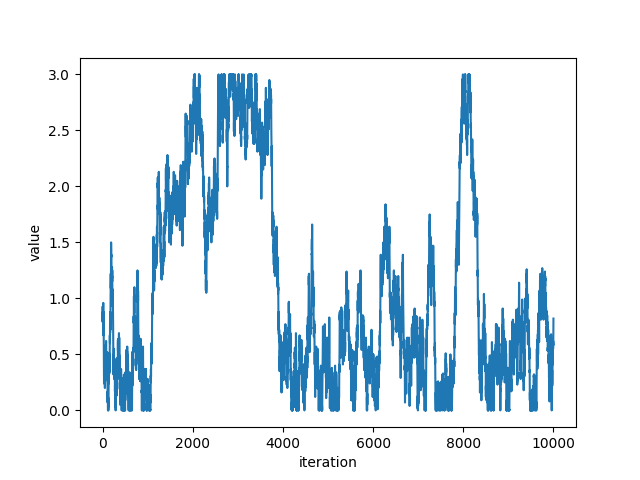
\includegraphics[width=\textwidth]{linechart_data_gen_dust10000i}
                                    \caption{For 10000 iterations}
                                    \label{chart:gen_dust_10000}
                                \end{subfigure}
                                
                                \caption{Sample generated dust sensor data }
                                \label{fig:gen_dust}
                        \end{figure}
                    \end{itemize}
                \subsection{Generated electricity voltage sensor data}
                        \begin{itemize}
                            \item Parameters
                                \begin{description}
                                    \item[Starting electricity voltage value:] 220
                                    \item[Minimum possible electricity voltage:] 208
                                    \item[Maximum possible electricity voltage:] 264
                                    \item[Maximum possible electricity change in an iteration:] 1
                                \end{description}
                            \item Results can be seen in figure \ref{fig:gen_voltage}
                                \begin{figure}
                                    \centering
                                    \captionsetup{type=figure}
                                    \begin{subfigure}[b]{0.45\textwidth}
                                        \centering
                                        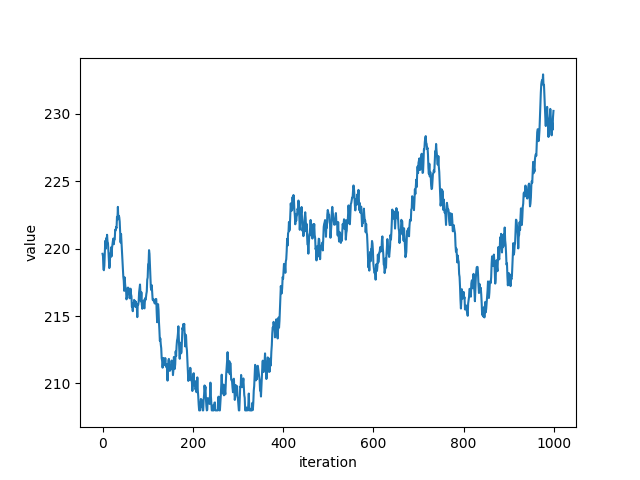
\includegraphics[width=\textwidth]{linechart_data_gen_voltage1000i}
                                        \caption{For 1000 iterations}
                                        \label{chart:gen_voltage_1000}
                                    \end{subfigure}
                                    \hfill
                                    \begin{subfigure}[b]{0.45\textwidth}
                                        \centering
                                        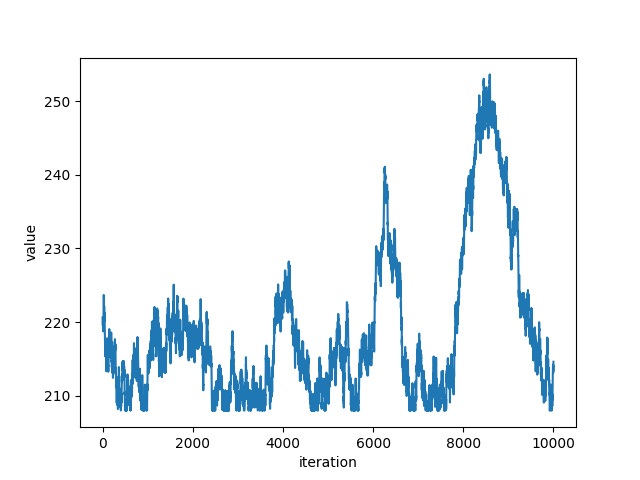
\includegraphics[width=\textwidth]{linechart_data_gen_voltage10000i}
                                        \caption{For 10000 iterations}
                                        \label{chart:gen_voltage_10000}
                                    \end{subfigure}
                                    
                                    \caption{Sample generated voltage sensor data }
                                    \label{fig:gen_voltage}
                            \end{figure}
                        \end{itemize}


                    \subsection{Generated electricity current sensor data}
                        \begin{itemize}
                            \item Parameters
                                \begin{description}
                                    \item[Starting electricity Current Value:] 220
                                    \item[Minimum possible electricity Current:] 208
                                    \item[Maximum possible electricity Current:] 264
                                    \item[Maximum possible change in an iteration:] 1
                                \end{description}
                            \item Results can be seen in figure \ref{fig:gen_voltage}
                                \begin{figure}
                                    \centering
                                    \captionsetup{type=figure}
                                    \begin{subfigure}[b]{0.45\textwidth}
                                        \centering
                                        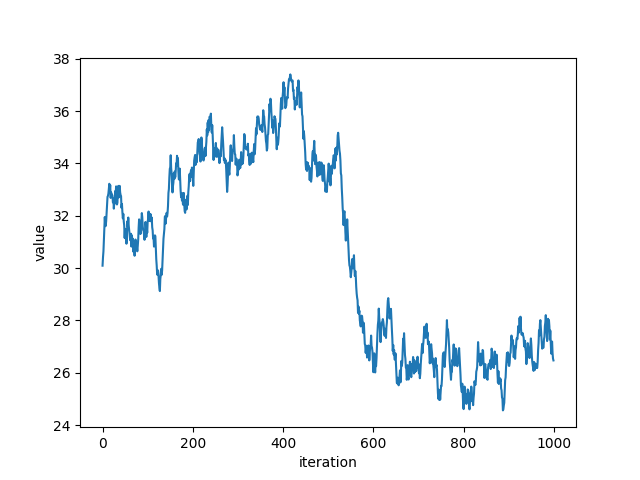
\includegraphics[width=\textwidth]{linechart_data_gen_current1000i}
                                        \caption{For 1000 iterations}
                                        \label{chart:gen_current_1000}
                                    \end{subfigure}
                                    \hfill
                                    \begin{subfigure}[b]{0.45\textwidth}
                                        \centering
                                        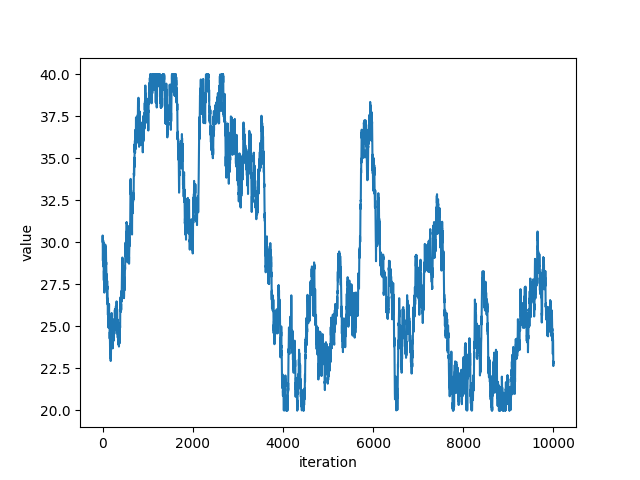
\includegraphics[width=\textwidth]{linechart_data_gen_current10000i}
                                        \caption{For 10000 iterations}
                                        \label{chart:gen_current_10000}
                                    \end{subfigure}
                                    
                                    \caption{Sample generated voltage sensor data }
                                    \label{fig:gen_voltage}
                            \end{figure}
                        \end{itemize}
        
